\documentclass[11pt]{article}
\usepackage{amsmath, amssymb, amscd, amsthm, amsfonts}
\usepackage{graphicx}
\usepackage{hyperref}
\usepackage{subfigure}
\usepackage{float}
\usepackage{rotating}
\usepackage{tikz}
\usepackage{xcolor}
\usepackage{listings}
\definecolor{vgreen}{RGB}{104,180,104}
\definecolor{vblue}{RGB}{49,49,255}
\definecolor{vorange}{RGB}{255,143,102}
\lstdefinestyle{verilog-style}
{
    language=Verilog,
    basicstyle=\small\ttfamily,
    keywordstyle=\color{vblue},
    identifierstyle=\color{black},
    commentstyle=\color{vgreen},
    numbers=left,
    numberstyle=\tiny\color{black},
    numbersep=10pt,
    tabsize=4,
    moredelim=*[s][\colorIndex]{[}{]},
    literate=*{:}{:}1
}

\makeatletter
\newcommand*\@lbracket{[}
\newcommand*\@rbracket{]}
\newcommand*\@colon{:}
\newcommand*\colorIndex{%
    \edef\@temp{\the\lst@token}%
    \ifx\@temp\@lbracket \color{black}%
    \else\ifx\@temp\@rbracket \color{black}%
    \else\ifx\@temp\@colon \color{black}%
    \else \color{vorange}%
    \fi\fi\fi
}
\makeatother

\usepackage{trace}



\oddsidemargin 0pt
\evensidemargin 0pt
\marginparwidth 40pt
\marginparsep 10pt
\topmargin -20pt
\headsep 10pt
\textheight 8.7in
\textwidth 6.65in
\linespread{1.2}

\title{NAND3 Simulation and Layout - Delay Analysis}
\author{Vladislav Pomogaev - 26951160}
\date{November 14, 2021}

\newcommand{\rr}{\mathbb{R}}

\newcommand{\al}{\alpha}
\DeclareMathOperator{\conv}{conv}
\DeclareMathOperator{\aff}{aff}

\begin{document}

\maketitle

\section{Problem 1}
\subsection{Specifications}
Here are the specifications for my NAND3 gate:
\begin{itemize}
\item Area: 0.0981 micrometer squared
\item Average delay: 25.61 pico-seconds
\item Area delay: 2.5130 pico-seconds micrometer squared
\end{itemize}

\begin{figure}[H]
	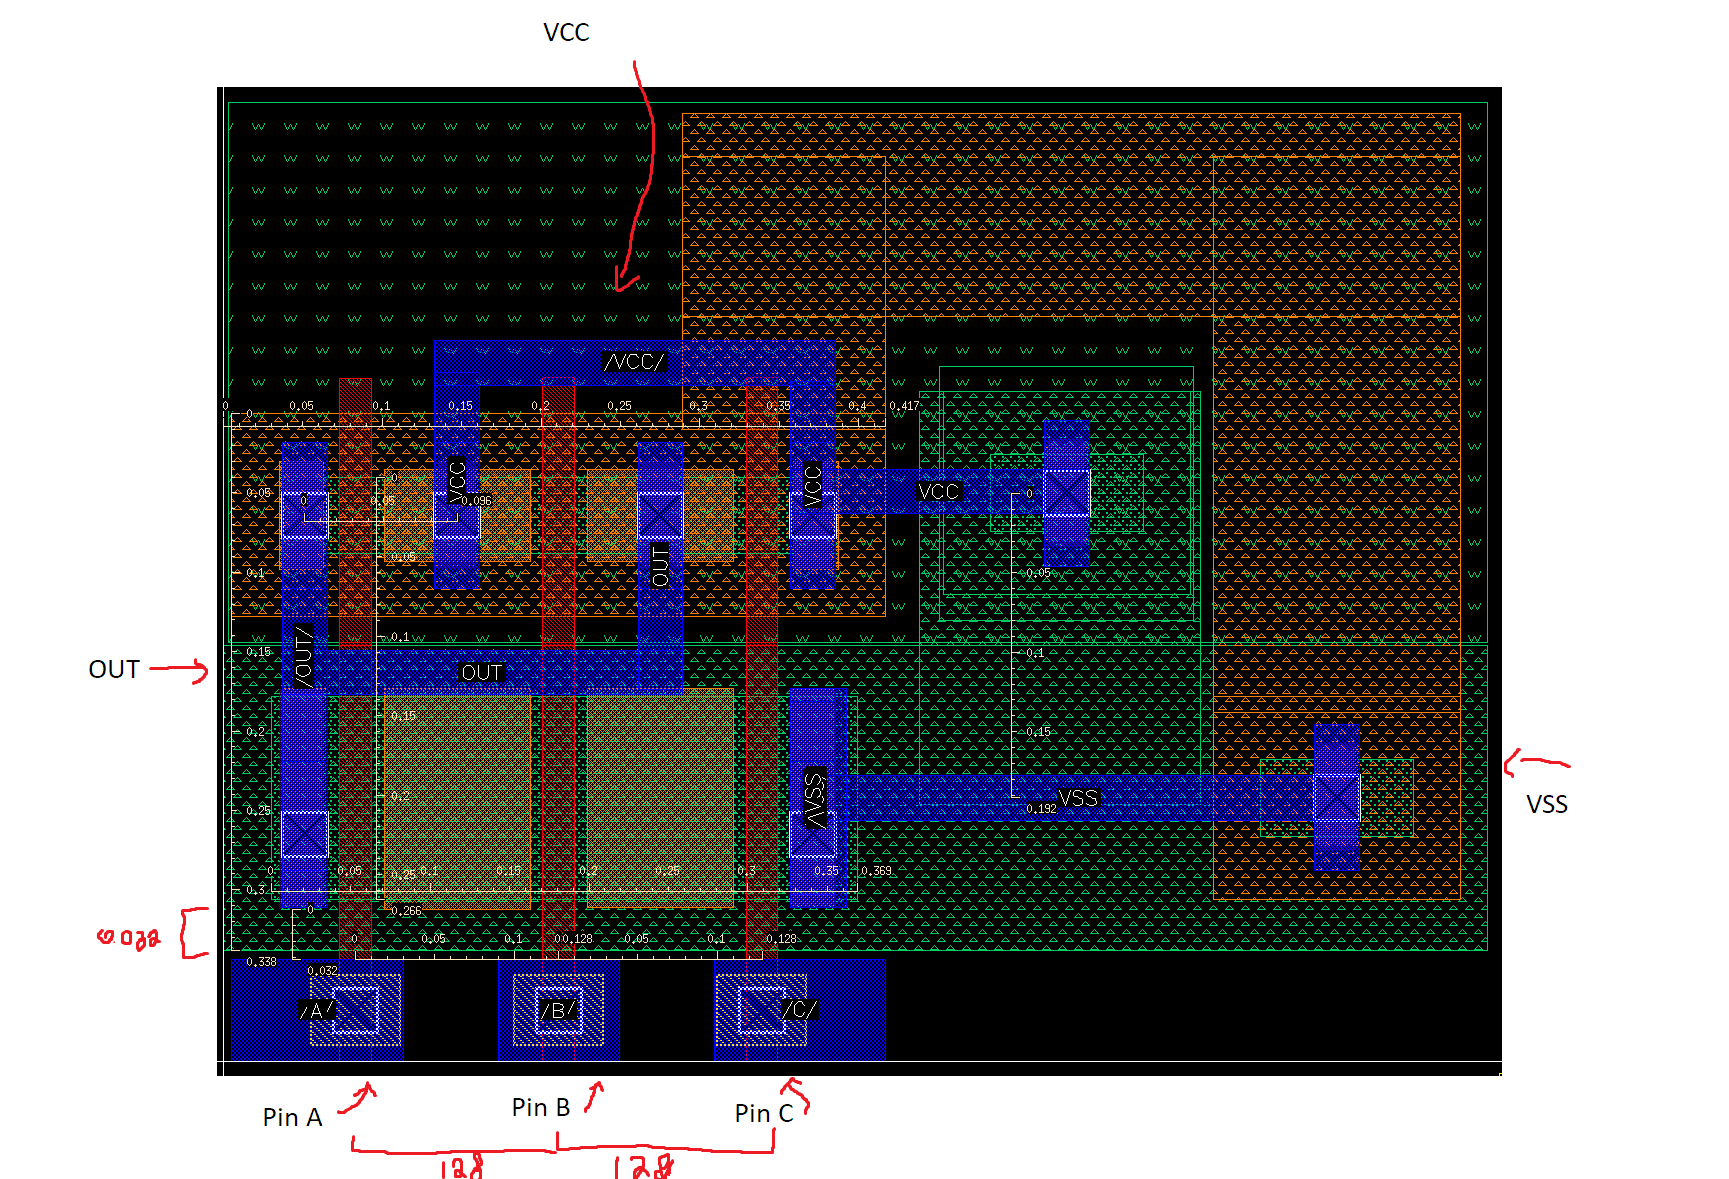
\includegraphics[width=0.98\textwidth]{layout_annot.png}
  	\caption{Layout of the gate. I had to add bulk connections otherwise I could not pass LVS for some reason. For the area, I measured the largest dimensions made by the active areas.}
\end{figure}

\begin{figure}[H]
  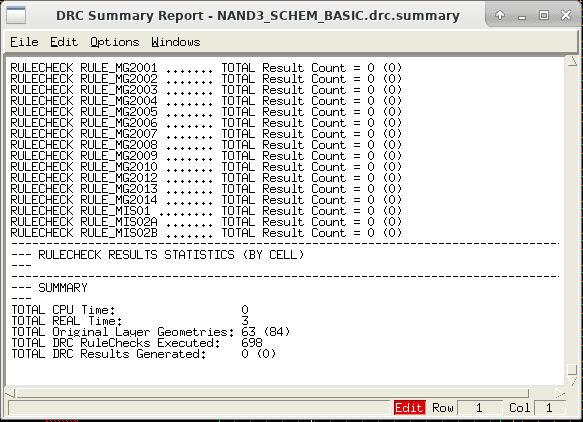
\includegraphics[width=0.98\textwidth]{drc.png}
  \caption{DRC Summary report (I solved the two rule checks that we were allowed to ignore)}
\end{figure}

\begin{figure}[H]
  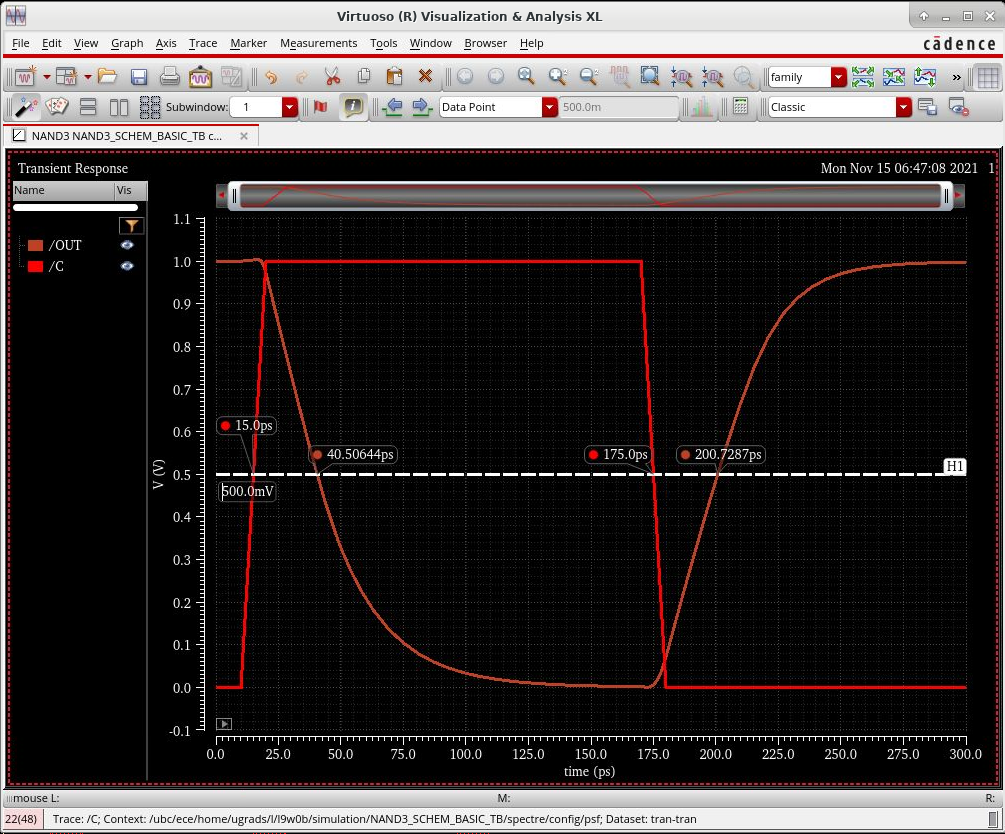
\includegraphics[width=0.98\textwidth]{timing.png}
  \caption{Timing of the gate. td,HL = 25.507ps, td,LD = 25.72ps. This graph was generated from the extracted view including all parasitics.}
\end{figure}

\begin{figure}[H]
  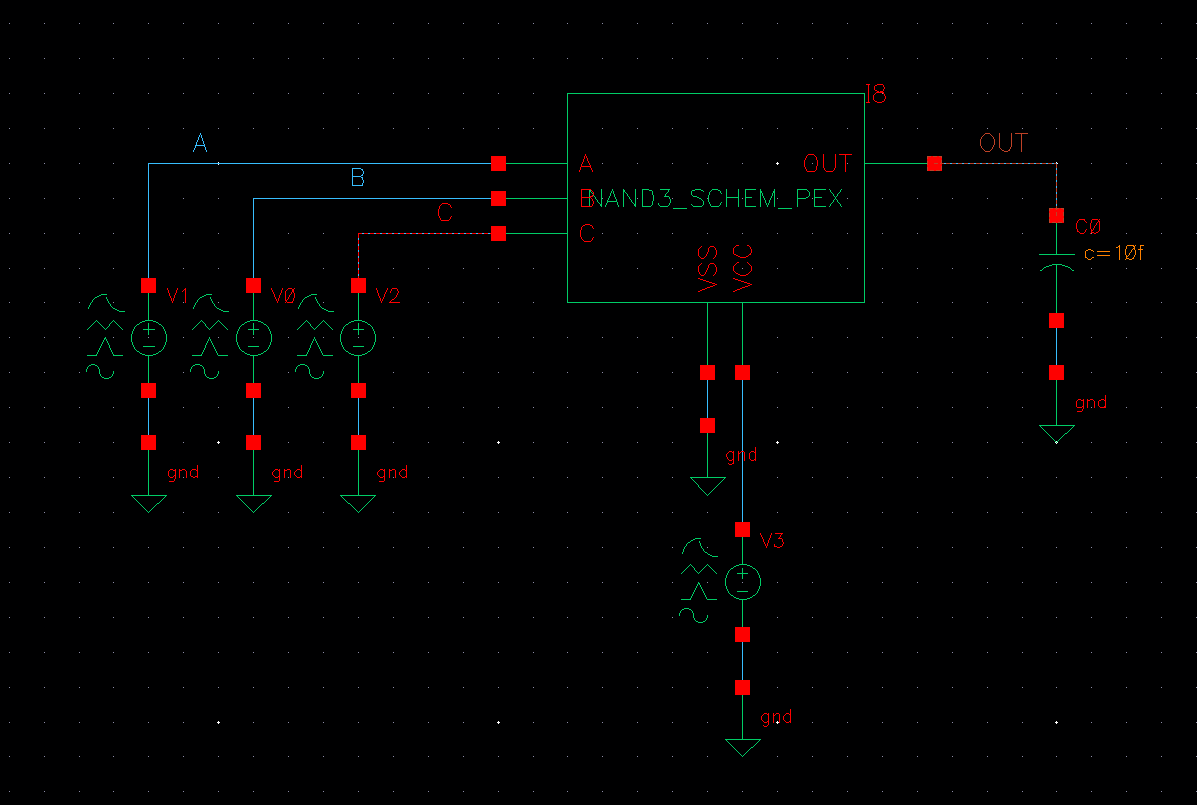
\includegraphics[width=0.98\textwidth]{schem.png}
  \caption{Screen-shot of my test bench schematic. I used a 10pF capacitor as the load. Worst-case switching was used (switching C, aka bottom n-fet results in worst switching).}
\end{figure}

\section{Problem 2}
\subsection{a)}
Using demorgan's law:
\[
\overline{F} = C D  (B + A)
\]
\[
\overline{\overline{F}} = \overline{C  D  (B + A)}
\]
\[
F = \overline{C} + \overline{D}  + \overline{B + A}
\]
\[
F = \overline{C} + \overline{D}  + \overline{B} \overline{A}
\]
\subsection{b)}

\subsection{c)}

\end{document}